\documentclass[11pt]{m2pi}
\usepackage{float}
\usepackage[backref=page]{hyperref}
\usepackage{xcolor}
\hypersetup{%
    colorlinks,
    linkcolor={red!60!black},
    citecolor={green!60!black},
    urlcolor={blue!60!black}
}

%%%%%%%%%%%%%%%%%%%%%%%%%%%%%%%%%%%%%%%%%%%%%%%%%%%%%%%%%%%%%%%%%%%%%%
%                          STANDARD PACKAGES                         %
%%%%%%%%%%%%%%%%%%%%%%%%%%%%%%%%%%%%%%%%%%%%%%%%%%%%%%%%%%%%%%%%%%%%%%

\usepackage{graphicx}
\graphicspath{{figures/}}

\usepackage{epstopdf}
\usepackage{amsthm}
\usepackage{amsmath}
\usepackage{amssymb}
\usepackage{amsxtra}
\usepackage{amscd}
\usepackage{verbatim}
\usepackage{rotating}
\usepackage{multirow}
\usepackage{multicol}
\usepackage{url}
\usepackage[margin=1.5in]{geometry}
\usepackage[all]{xy}

%%%%%%%%%%%%%%%%%%%%%%%%%%%%%%%%%%%%%%%%%%%%%%%%%%%%%%%%%%%%%%%%%%%%%%
%                        STANDARD ENVIRONMENTS                       %
%%%%%%%%%%%%%%%%%%%%%%%%%%%%%%%%%%%%%%%%%%%%%%%%%%%%%%%%%%%%%%%%%%%%%%

% Theorems

%Commented out this theorem style I  have no idea why it's even here - Erik
%\theoremstyle{theorem}
\newtheorem{theorem}{Theorem}[section]
\newtheorem{alphtheorem}{Theorem}
\renewcommand{\thealphtheorem}{\Alph{alphtheorem}}
\newtheorem{lemma}[theorem]{Lemma}
\newtheorem{corollary}[theorem]{Corollary}
\newtheorem{guess}[theorem]{Conjecture}
\newtheorem{definition}[theorem]{Definition}
\newtheorem{facts}[theorem]{Facts}
\newtheorem{proposition}[theorem]{Proposition}
\newtheorem{problem}[theorem]{Problem}
%\newtheorem{algorithm}[theorem]{Algorithm}
%\newtheorem{claim}{Claim}[theorem]
\newtheorem{claim}[theorem]{Claim}
\newtheorem{subclaim}{Claim}[theorem]
\renewcommand{\thesubclaim}{\thetheorem.\alph{subclaim}}
\newtheorem{example}[theorem]{Example}
%\newtheorem*{example*}{Example}
\newtheorem{result}[theorem]{Result}
\newtheorem{observation}[theorem]{Observation}
\newtheorem{numconjecture}[theorem]{Conjecture}

\newtheoremstyle{myexample}{3pt}{3pt}{}{}{\bfseries}{.}{ }{\thmname{#1}\thmnumber{ #2}\thmnote{ (#3)}}
\theoremstyle{myexample}
\newtheorem{numremark}[theorem]{Remark}

\newtheoremstyle{myremark}{3pt}{3pt}{}{}{\bfseries}{.}{ }{\thmname{#1}\thmnote{ (#3)}}
\theoremstyle{myremark}
\newtheorem{remark}{Remark}
\newtheorem*{remark*}{Remark}
\newtheorem*{remarks*}{Remarks}
\newtheorem*{observation*}{Observation}
\newtheorem*{example*}{Example}

\newtheoremstyle{conjecture}{3pt}{3pt}{\itshape}{}{\bfseries}{.}{ }{\thmname{#1}\thmnote{ (#3)}}
%\newtheoremstyle{conjecture}{3pt}{3pt}{\rmfamily}{}{\itshape}{.}{ }{\thmname{#1}}
\theoremstyle{conjecture}
\newtheorem{question}{Question}
\newtheorem*{question*}{Question}
\newtheorem{conjecture}{Conjecture}
\newtheorem{theorem*}{Theorem}


\numberwithin{equation}{section}

% References
\newcommand{\genericref}[2]{#1~\ref{#2}}
\newcommand{\generictworef}[3]{#1~\ref{#2} and \ref{#3}}
\newcommand{\genericthreeref}[4]{#1~\ref{#2}, \ref{#3} and \ref{#4}}
\newcommand{\thmref}[1]{\genericref{Theorem}{#1}}
\newcommand{\lemmaref}[1]{\genericref{Lemma}{#1}}
\newcommand{\claimref}[1]{\genericref{Claim}{#1}}
\newcommand{\remarkref}[1]{\genericref{Remark}{#1}}
\newcommand{\conjref}[1]{\genericref{Conjecture}{#1}}
\newcommand{\tableref}[1]{\genericref{Table}{#1}}
\newcommand{\figref}[1]{\genericref{Figure}{#1}}
\newcommand{\twofigref}[2]{\generictworef{Figures}{#1}{#2}}
\newcommand{\threefigref}[3]{\genericthreeref{Figures}{#1}{#2}{#3}}
\newcommand{\propref}[1]{\genericref{Proposition}{#1}}
\newcommand{\twopropref}[2]{\generictworef{Propositions}{#1}{#2}}

% Case environment
\newenvironment{genericcase}[6]{\medskip\par\noindent \csname#1\endcsname{#2 #3}#4 \csname#5\endcsname{#6}.\begin{indentation}{1.5em}{0em}\noindent\ignorespaces}{\end{indentation}}
\newenvironment{case}[2]{\noindent \textit{Case #1}: #2.\begin{indentation}{1.5em}{0em}}{\end{indentation}}

%Note that I changed  \textit{Subcase #1}. #2. to  \textit{Subcase #1}: #2.
%Erik

\newenvironment{subcase}[2]{\noindent \textit{Subcase #1}: #2.\begin{indentation}{1.5em}{0em}}{\end{indentation}}
\newenvironment{ulindent}[1]{\noindent \underline{#1:}\begin{indentation}{1.5em}{0em}\setlength{\parindent}{0em}}{\end{indentation}}
\newenvironment{bfcase}[1]{\par\medskip\begin{indentation}{1.5em}{0em}\noindent\hspace*{-1.5em}\textbf{#1:}}{\end{indentation}}
\newenvironment{itcase}[1]{\par\medskip\begin{indentation}{1.5em}{0em}\noindent\hspace*{-1.5em}\textit{#1:}}{\end{indentation}}
%\newcommand{\case}[2]{\noindent \textbf{Case #1}: #2:}

% Induction environment
\newenvironment{basecase}[1]{\noindent \textsc{Base case}: #1:\begin{indentation}{1.5em}{0em}}{\end{indentation}}
\newenvironment{inductionstep}[1]{\noindent \textsc{Induction step}: #1:\begin{indentation}{1.5em}{0em}}{\end{indentation}}

% Algorithm headers
\newcounter{algorithm}
\setcounter{algorithm}{0}
\renewcommand{\thealgorithm}{\thesection.\arabic{algorithm}}
\newenvironment{algorithm}[1]{%
  \null
  \refstepcounter{algorithm}%
  \hrule%
  \vspace{0.2em}%
  \noindent\textbf{Algorithm \thealgorithm} #1
  \vspace{0.2em}%
  \hrule%
  \vspace{0.2em}
  }{%
  \vspace{0.2em}%
  \hrule%
  \null
}

%%%%%%%%%%%%%%%%%%%%%%%%%%%%%%%%%%%%%%%%%%%%%%%%%%%%%%%%%%%%%%%%%%%%%%
%                          STANDARD COMMANDS                         %
%%%%%%%%%%%%%%%%%%%%%%%%%%%%%%%%%%%%%%%%%%%%%%%%%%%%%%%%%%%%%%%%%%%%%%

\newcommand{\ie}{i.e.}
\newcommand{\eg}{e.g.} 
\newcommand{\resp}{\emph{resp.\@\ }} 
\newcommand{\etal}{et~al.} 
\newcommand{\cf}{cf.}

\newcommand{\mathbif}[1]{\mathbf{\emph{#1}}}
\newcommand{\nth}[1]{\ensuremath{#1^{\textrm{th}}}}
\newcommand{\nrd}[1]{\ensuremath{#1^{\textrm{rd}}}}
\newcommand{\nst}[1]{\ensuremath{#1^{\textrm{st}}}}
\newcommand{\jth}{\nth{j}}
\newcommand{\kth}{\nth{k}}
\newcommand{\qth}{\nth{q}}
\newcommand{\rth}{\nth{r}}

\newcommand{\vfrac}[2]{\ensuremath{{}^{\displaystyle#1} \diagup {}_{\displaystyle#2}}}

\renewcommand{\pmod}[1]{\ \left({\rm mod\ } #1 \right)}

%%%%%%%%%%%%%%%%%%%%%%%%%%%%%%%%%%%%%%%%%%%%%%%%%%%%%%%%%%%%%%%%%%%%%%
%                      SAVING THEOREM NUMBERS                        %
%%%%%%%%%%%%%%%%%%%%%%%%%%%%%%%%%%%%%%%%%%%%%%%%%%%%%%%%%%%%%%%%%%%%%%

%\newcounter{temp}
%\def\savecounter#1{\newcounter{#1}\setcounter{#1}{\value{theorem}}}
%\def\changetheoremcounter#1{\setcounter{temp}{\value{theorem}}\setcounter{theorem}{\value{#1}}}%\csname the#1\endcsname}}
%\def\restoretheoremcounter{\setcounter{theorem}{\value{temp}}}

\newcounter{temp}
\newcounter{ctemp}
\def\savecounter#1#2{%
   \newcounter{#1}%
   \setcounter{#1}{\value{section}}%
   \newcounter{#2}\setcounter{#2}{\value{theorem}}}
\def\swapcounter#1#2{%
   \setcounter{ctemp}{\value{section}}%
   \setcounter{section}{\value{#1}}%
   \setcounter{temp}{\value{theorem}}%
   \setcounter{theorem}{\value{#2}}%
   \addtocounter{theorem}{-1}}
\def\restorecounter{%
   \setcounter{section}{\thectemp}%
   \setcounter{theorem}{\thetemp}}

\usepackage{subfigure}% in preamble
%\usepackage{lineno}
%\linenumbers

\newcommand{\eps}{\varepsilon}
\newcommand{\vf}{\varphi}
\newcommand{\cP}{\mathcal{P}}
\newcommand{\cH}{\mathcal{H}}
\newcommand{\cL}{\mathcal{L}}
\newcommand{\cM}{\mathcal{M}}
\newcommand{\cB}{\mathcal{B}}
\newcommand{\cD}{\mathcal{D}}
\newcommand{\cF}{\mathcal{F}}
\newcommand{\cO}{\mathcal{O}}
\newcommand{\cS}{\mathcal{S}}
\newcommand{\cN}{\mathcal{N}}
\newcommand{\cT}{\mathcal{T}}
\newcommand{\cU}{\mathcal{U}}
\newcommand{\fD}{\mathfrak{D}}
\newcommand{\fX}{\mathfrak{X}}
\newcommand{\fS}{\mathfrak{S}}
\newcommand{\bF}{\mathbb{F}}
\newcommand{\bH}{\mathbb{H}}
\newcommand{\bP}{\mathbb{P}}
\newcommand{\bR}{\mathbb{R}}
\newcommand{\bN}{\mathbb{N}}
\newcommand{\bS}{\mathbb{S}}
\newcommand{\bL}{\mathbb{L}}
\newcommand{\sF}{\mathscr{F}}
\newcommand{\sJ}{\mathscr{J}}
\newcommand{\sL}{\mathscr{L}}
\newcommand{\sS}{\mathscr{S}}
\newcommand{\sB}{\mathscr{B}}
\newcommand{\sA}{\mathscr{A}}
\newcommand{\sH}{\mathscr{H}}
\newcommand{\sP}{\mathscr{P}}
\newcommand{\la}{\langle}
\newcommand{\ra}{\rangle}
\newcommand{\intl}{\interleave}
\newcommand{\rrow}{\rightarrow}
\newcommand{\tbf}{\textbf}
\newcommand{\ves}{\varepsilon}

\begin{document}

\title{Modelling Canadian heavy crude congestion pricing}

\author[M. Azizi]{Mahsa Azizi}
\address{University of Saskatchewan, Dept. of Computer Science, Thorvaldson Building, Saskatoon SK, S7N 5C9, Canada}
\email{mahsa.azizi@usask.ca}

\author[E. Chan]{Erik Chan}
\address{University of Calgary, Dept. of Math. and Stat.
2500 University Drive NW, Calgary AB, T2N 1N4, Canada}
\email{erik.chan@ucalgary.ca}

\author[X. Fu]{Xilai Fu}
\address{University of Alberta, Dept. of Math. and Stat. 11840 90 St NW, Edmonton AB, T5B 3Y6, Canada}
\email{xilai@ualberta.ca}

\author[N. Safaian]{Nima Safaian}

\author[S. P. Torabi]{S. Parisa Torabi}
\address{Brock University, Dept. of Physics. 500 Glenridge Avenue, St. Catharines On,  L2S 3A1, Canada}
\email{sparisatorabi@gmail.com}

\author[W. Wei]{Wenning Wei}
\address{University of Calgary, Dept. of Math. and Stat.
2500 University Drive NW, Calgary AB, T2N 1N4, Canada}
\email{wenning.wei@ucalgary.ca}

\begin{abstract}
In this brief report, we establish a mixed-integer, linear programming model to estimate the congestion surcharge from price spread for crude oil prices over a fixed transport network with one or more consumer nodes. For the one node model, the North American crude oil market is discussed. Pseudo data simulated by an Ornstein-–Uhlenbeck stochastic process is used to study the multi-node model.
\end{abstract}


\maketitle

\section{Introduction}
Spatial price integration in oil commodity markets studies the price movement in the market between market participants that are geographically separated. Crude oil markets are generally considered well-integrated as the different types of oil (e.g., light and heavy oil) are fungible assets and there is a vast network of pipelines and train capacity available to deliver oil efficiently to its destination.

There are many different classifications of oil commodities on the global market separated by variables such as viscosity and sulphur content. Among them, we focus on West Texas Intermediate (WTI), a high-quality oil priced out of Cushing, Oklahoma which serves as the primary benchmark in North America, and Western Canada Select (WCS), Canada's largest heavy oil stream.

Alberta produces approximately 4 million barrels per day (MMb/d) of crude oil of which approximately 3 MMb/d is classified as heavy oil. The majority of WCS is consumed in the Midwestern United States with the remaining excess stock destined for domestic consumption sent to the US Gulf Coast, see \cite{Hackett}. The US Gulf Coast is considered as a marginal consumption point where the last barrel is consumed. Canadian crude oil can reach the Gulf Coast through different pipeline options or rail from Edmonton or Hardisty, Alberta. The transportation cost of the last barrel to the Gulf Coast sets the price of WCS.

\begin{figure}[h!]
    \centering
    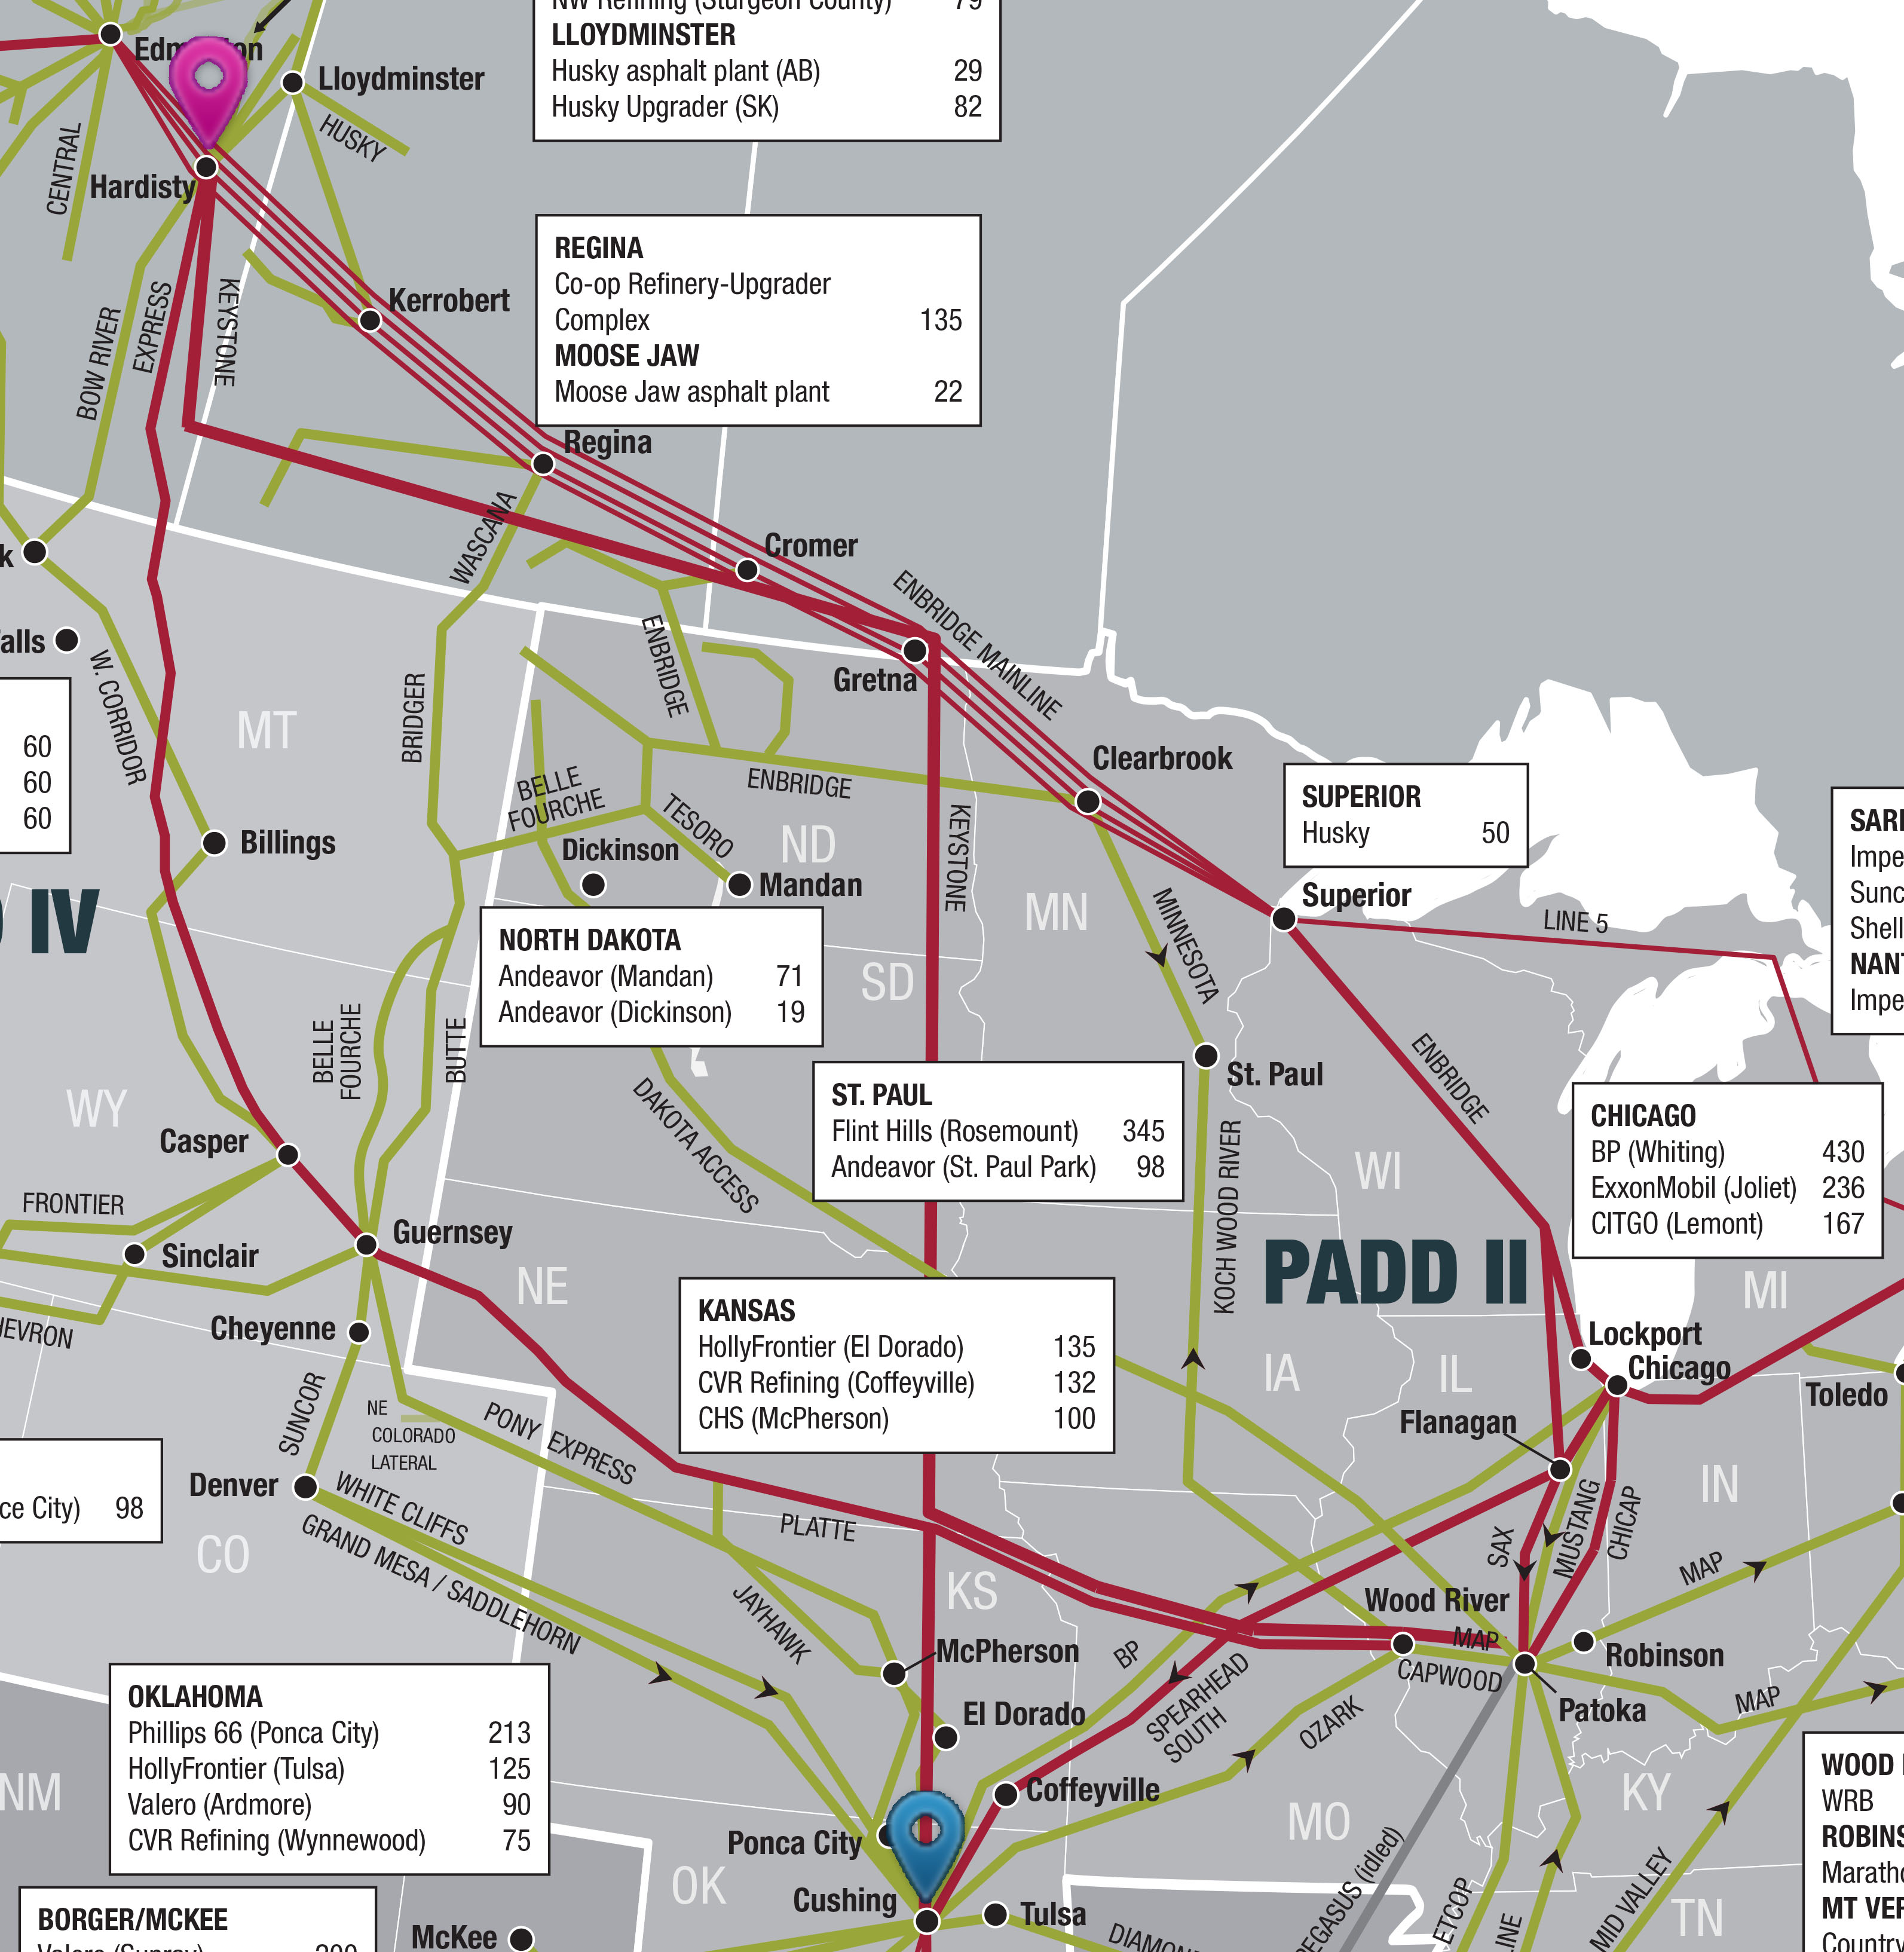
\includegraphics[scale=0.40]{map5.jpg}
    \caption{Map of crude oil pipelines~\cite{pipelineMap}. The pink marker is located at Hardisty, Alberta and the blue marker is located at Cushing, Oklahoma.}
    \label{fig:PADD Map}
\end{figure}


The total off-take capacity of the pipeline from Alberta is on average less than the supply, this leads to ``call-on-rail'' (using expensive rail to transport oil) or shut-ins (mandatory curtailment of oil production). The price response to this supply-capacity difference is significant and appears as a regular breakdown in the price relationship between WCS and WTI that we define as a period of congestion pricing. This is exasperated by periods of congestion leading to the formation of transient ``submarkets''.


\subsection{Documented congestion}

In the first half of 2018, western Canadian heavy oil production increased steadily while pipeline capacity did not increase. As a result, some production was shifted to rail, which is more expensive. Consequently, Canadian crude benchmarks faced large price discounts, and the difference between WCS and WTI increased compared to 2017 \cite{disruption2018}.

In the second half of 2018, the WCS—-WTI differential widened more than normal. The reason behind that was the supply of western Canadian oil production rose to 4.30 MMb/d while takeaway capacity on existing pipelines remained constant at around 3.95 MMb/d. Moreover, the demand from the United States decreased due to the shutdown of some refineries in the Midwest for maintenance, which is the largest export market for Canadian heavy crude oil \cite{CER2018}.

Canadian crude oil exports via pipeline increased $3\%$ from $3.1$ MMb/d in 2018 to $3.2$ MMb/d in 2019. At the same time, exporting crude oil via rail increased by $16\%$ from 2018 to 2019. This growth in rail exports was largely due to pipeline capacity constraints in the Western Canada Sedimentary Basin \cite{CER2019}. Also, on October 28, 2019, around $9,120$ barrels of oil were leaked from the Keystone pipeline causing a shut down for ten days \cite{CNN2019}.

In 2020, due to the COVID-19 pandemic, some activities such as travelling were restricted in countries around the world to reduce the spread of the disease. The demand for Canadian crude oil products decreased significantly and the Canadian energy sector shut down production as low crude oil prices persisted \cite{CER2020}. The reduced supply removed pipeline capacity constraints in the transportation network and reduced the price spread between WTI and WCS as a consequence.
\begin{figure}[h!]
    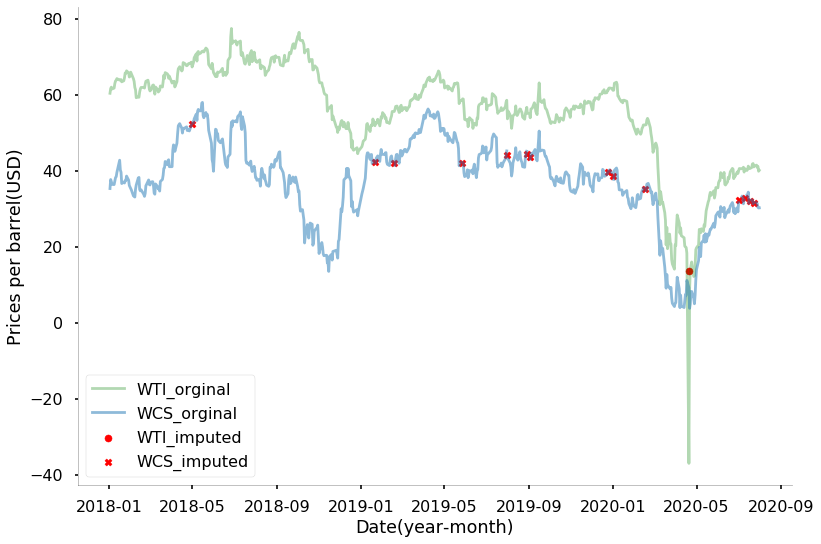
\includegraphics[width=\textwidth]{WTS_WCS_updated.png}
    \caption{The price of WTI and WCS from January 2018, to August 2020. Missing data in WCS is filled-in using the average of its nearest neighbours. An outlier (-37USD) in WTI at Apr. 20, 2020 is replaced by interpolation.}
    \label{fig:spread}
\end{figure}
\subsection{Main result}
In this report, in collaboration with Cenovus Energy Inc., we build a mixed-integer linear (MIL) programming model to estimate the congestion surcharge from the price spread between different geographic regions over a transportation network connecting consumers and producers.

We start with a baseline model with a single consumer node that only considers the price spread between Hardisty and Cushing in 2018--2020. Taking Hardisty as the producer node and Cushing as the consumer node, we detect periods of congestion and the associated surcharge during this period and show that this model matches documented periods of congestion well. We then extend the model to multiple consumer nodes, simulate price data using an Ornstein–Uhlenbeck (OU) stochastic process (calibrated using historical WTI--WCS spot prices) over a network of consumers (refineries) in the absence of sufficient real-world data, and estimate the time and value the congestion surcharge. 

This report consists of the following sections. In section two, a mixed-integer, linear programming model is established for a transportation network to estimate congestion. In section three, the one-node model is used to study the North American crude oil market for crude oil travelling from Alberta to the United States. In section four, a general multi-consumer model is applied to simulated data from an OU process. In section five, a summary of the results and possible future research are discussed.

\section{A mathematical model for congestion surcharge}
In \cite{Zhu2020}, Birge et al.~shows that in an equilibrium integrated market, the price of a commodity at different locations can be decomposed into a baseline price for the commodity, a transportation cost, a congestion surcharge, and a variable contained by a \emph{neutral band} of values the local equilibrium price can take without exhibiting arbitrage due to transportation costs, see Lemma~\ref{lemma:decomposition}.

We denote by $\cT$, a set of times measured in days, and $\cS$, a set of consumer nodes over a transportation network connecting the nodes $\cS$ to some collection of producers. Note that each consumer node may represent a cluster of nodes in close spatial proximity, such as all consumers residing in the same city.

\begin{lemma}[{\cite[Proposition 3]{Zhu2020}}]\label{lemma:decomposition}
The set of equilibrium prices $\{\lambda_s^t,~~\,\forall s\in\cS,\,\forall t\in\cT\}$ over a market with fixed transportation network structure and transportation (link) costs can be decomposed into
\[\lambda_s^t = \eta^t+\rho_s+\ves_s^t +\omega_s^t,\quad \forall s\in\cS,\,t\in\cT,\]
\end{lemma}

In this lemma, $\ves_s^t\in[-\alpha_s, \alpha_s]$ represents the neutral band, $\eta^t$ is the baseline price for the commodity taken to be the spot price at a neutral node unaffected by congestion, and $\omega_s^t\geq 0$ is the congestion surcharge. 

In our model, we set $\eta_t$ to be the equilibrium price of the producer (assumed to be at a single node). Then, the formula in Lemma \ref{lemma:decomposition} reduces to 
\[\xi_s^t = \rho_s + \ves_s^t +\omega_s^t\] where $\xi^t_s = \lambda_s^t - \eta^t$ denotes the price spread between consumer $s$ and producer. 

Therefore, to estimate the congestion surcharge in the transportation network, we construct the following mixed-integer, linear programming problem.  

\begin{align}\label{1}
\text{minimize: } &\sum_{s\in\cS} \alpha_s\\
\text{subject to: } &\xi_s^t = \rho_s + \ves_s^t +\omega_s^t,\quad \forall \nonumber s\in\cS,t\in\cT,\\ \nonumber
&-\alpha_s\leq\ves_s^t \leq \alpha_s,\quad \forall s\in\cS,t\in\cT,\\ \nonumber
&0\leq\omega_s^t\leq \gamma_s^t M,\quad \forall s\in\cS,t\in\cT,\\ \nonumber
&\ves_s^t \geq \alpha_s - (1-\gamma_s^t) M,\quad \forall s\in\cS,t\in\cT,\\ \nonumber
&\psi^t\leq\sum_s \gamma_s^t\leq |\cS|\, \psi^t, \quad \forall t\in\cT,\\ \nonumber
&\sum_t \psi^t \leq \beta T, \quad \forall t\in\cT,\\ \nonumber
&\psi^t, \gamma_s^t \in\{0,1\}, \quad \forall s\in\cS,t\in\cT.\\ \nonumber
\end{align}
Here $\xi_{s}^{t}$ denotes the price spread between the price of the commodity at the consumer node $s$ and the producer, $M$ is a sufficiently large upper bound for the congestion surcharge, $\psi$ (resp.~$\gamma$) is an indicator function taking the value $1$ representing congestion in the network (resp.~representing congestion at $s$) and taking the value 0 in the absence of congestion (resp.~ in the absence of congestion at $s$). Finally, $\beta\in[0,1]$ is a fixed parameter set by the user that represents the proportion of the time that congestion is allowed to manifest, i.e., time periods when the surcharge term $\omega_s^t$ can take positive values. 

When there is only one consumer node in $\mathcal{S}$, the above mixed-integer, linear programming problem is simplified to 

\begin{align}\label{2}
\text{minimize: } &\alpha\\ \nonumber
\text{subject to: } &\lambda^t = \rho + \ves^t +\omega^t, \quad \forall t\in\cT,\\\nonumber
&-\alpha\leq\ves^t \leq \alpha,\\\nonumber
&0\leq\omega^t\leq \psi^t M,\\\nonumber
&\ves^t \geq \alpha - (1-\psi^t) M,\\ \nonumber
&\sum_t \psi^t \leq \beta T,\\\nonumber
&\psi^t \in\{0,1\},\nonumber
\end{align}
i.e., $\gamma$ is no longer necessary since the parameter determines which node experiences congestion conditional on congestion occurring somewhere on the network.

\section{Congestion surcharges in the crude oil market}
In this section, we use the above programming model to estimate the congestion surcharge in the crude oil market in North America. We analyze WCS from Hardisty, Alberta and WTI from Cushing Oklahoma. We take Hardisty as the producer node with WCS as the local price, and Cushing to be the consumer node with a local price set to be \$5 lower than the WTI spot price to account for the difference between heavy and light oil. See The spot price data between WCS and WTI from January 2018 to August 2020 can be found in Figure~\ref{fig:spread}. 




Using model \eqref{2}, we set the price spread to be WTI$-$WCS$-5$ as described above, set $M=100$ as an arbitrarily large upper bound for the congestion surcharge, and for $\beta \in \{0.2,~0.4,~0.6,~0.8\}$, we get the congestion surcharges shown in Figure~\ref{fig:Congestion Surcharge}. The pink shaded regions represent time periods with documented pipeline disruption or “call-on-rail”, while the green shaded region corresponds to a period with sufficient pipeline capacity but with reduced demand. Therefore, we can see that selecting $\beta=0.4$ or $\beta = 0.6$, the congestion surcharge estimated by the model seems to match the market well.
%%%%%%%%%%%%%%%%%%%%%%%%%%%%%%%%%%%%%%%%%%%%%%
% Put Congestion Surcharge Figure in section 3
% \label{fig:Congestion Surcharge}
%%%%%%%%%%%%%%%%%%%%%%%%%%%%%%%%%%%%%%%%%%%%%%
\begin{figure}[h!]
    \centering
    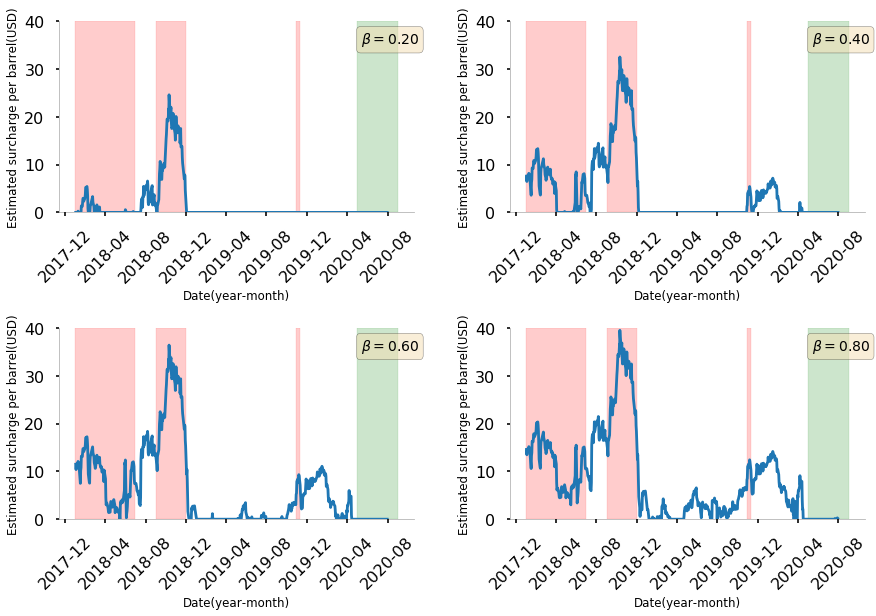
\includegraphics[width = \linewidth]{image8.png}
    \caption{Estimated congestion surcharge for a single consumer node with different choices of $\beta$. Periods of historical congestion are denoted by the pink shaded regions and a period of decreased demand is denoted by the green shaded region.}
    \label{fig:Congestion Surcharge}
\end{figure}

\section{Multi-node model with pseudo data}
In this section, we estimate the congestion surcharge in a transportation network with one producer node and several consumer nodes. Due to the lack of data, we simulate price spreads by using three correlated OU processes for the consumer nodes following the stochastic differential equation,
\[\operatorname{d}\!x_t  = \alpha(\mu-x_t)\,\operatorname{d}\!t + \sigma \operatorname{d}\!W_t.\].

The parameters $\alpha, \mu,$ and $\sigma$ for the OU process are calibrated using the WTI--WCS spread spot price. Using the method of maximum likelihood estimation, we obtain the following parameters: $\alpha=0.0119$, $\mu=16.275$, $\sigma=2.053$.
These parameters and three correlated Brownian motions following the correlation matrix
\[\operatorname{corr} = 
    \begin{bmatrix}
    1& 0.8& 0.7\\
    0.8& 1 &0.56\\
    0.7 & 0.56 &1
    \end{bmatrix},
\]
are used to simulate three sample price spreads for the three refineries and the one producer. See Figure~\ref{SimSpread}.

\begin{figure}[ht]
    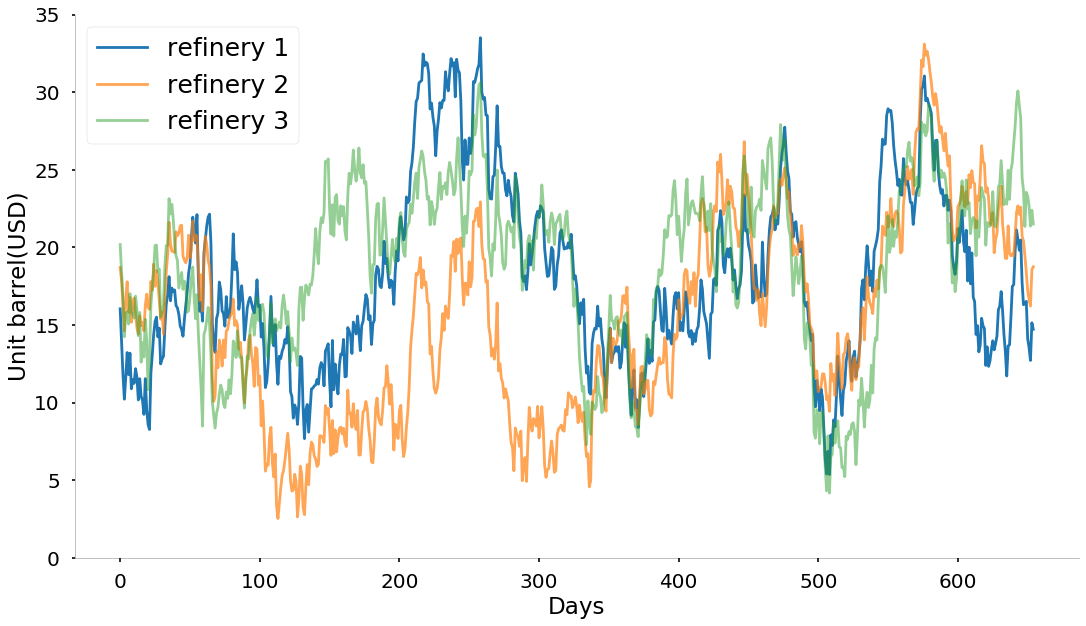
\includegraphics[width=\linewidth]{refinery.png}
    \caption{Simulated paths for three refineries (consumer nodes $s\in \mathcal{S}$)}\label{SimSpread}
\end{figure}

Using model \eqref{1} with $\cS$ containing three consumer nodes, the congestion surcharge for $\beta\in \{0.2,0.4,0.6,0.8\}$ are simulated in Figure~\ref{fig:minipage1}.



\begin{figure}[h!]
	\centering
	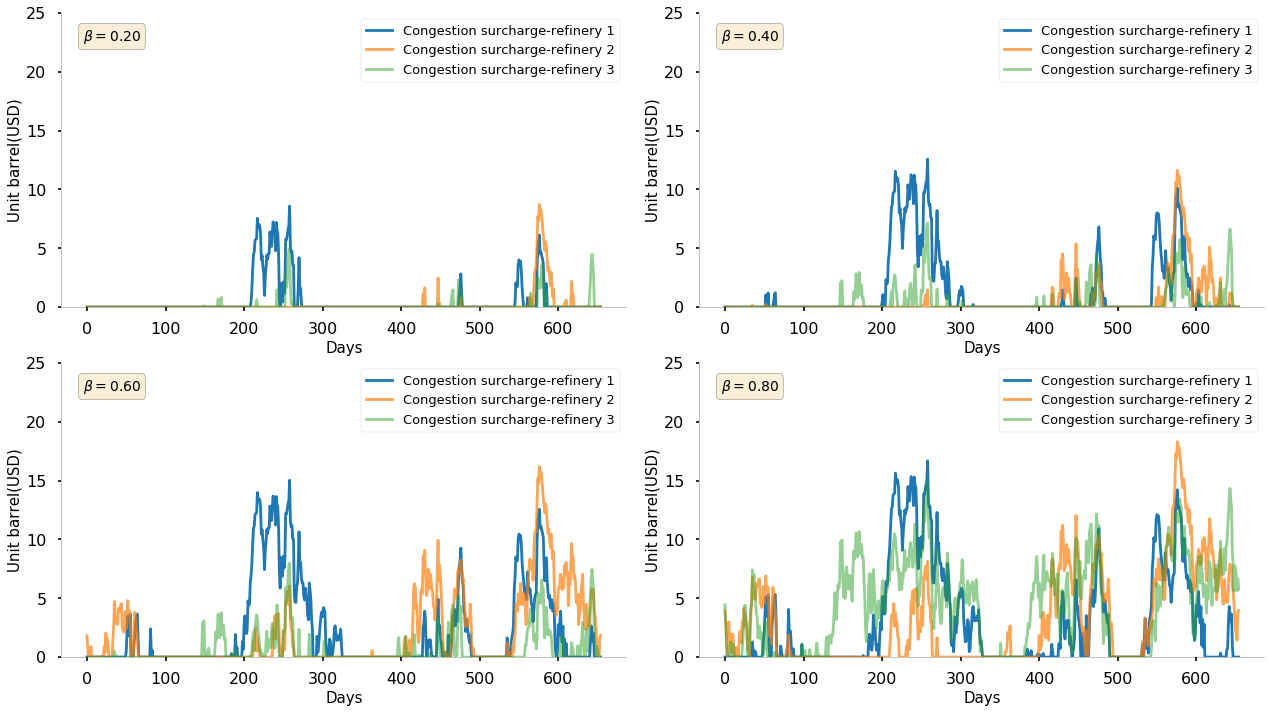
\includegraphics[width=\linewidth]{multinode with beta.png}
	\caption{Multi-node congestion surcharges for three refineries with different choices of $\beta$.}\label{fig:minipage1}
\end{figure}



\section{Conclusion}
In this project, we were able to successfully identify periods of historical congestion from 2018 to 2020 using a mixed-integer, linear programming model by studying the spread price between WTI and WCS. We further generalized the model to a multi-node model. This multi-node model can be used to further examine the graph-theoretic shape of the crude oil market by adding and removing refineries to study the behaviour of congestion before and after changes are made to the network structure.
\section*{Acknowledgements}
We wish to thank Nima Safaian for his support and guidance throughout this project. We would like to further thank PIMS for organizing a wonderful workshop.
\bibliographystyle{amsplain}
\bibliography{project}

\end{document}
